\begin{savequote}[8cm]
\textlatin{Neque porro quisquam est qui dolorem ipsum quia dolor sit amet, consectetur, adipisci velit...}

There is no one who loves pain itself, who seeks after it and wants to have it, simply because it is pain...
  \qauthor{--- Cicero's \textit{de Finibus Bonorum et Malorum}}
\end{savequote}

\chapter{\label{ch:7-com}Centre-of-momentum variables} 

    Inspired by the kinematic measurement of hadrons, I have constructed a set of new variables specific to the $\numuccopi$-Trackless sample and I call them the centre-of-momentum (COM) variables. 
    The key idea is to reconstruct the $\deltapp$ momentum using only hadronic variables.  

    The $\numuccopiop$ sample contains mostly resonance reaction, where the proton and the pion are the decay products of the $\deltapp$. 
    Without FSI, the sum, $\vecpsum$, of the proton momentum, $\vecpp$, and the pion momentum, $\vecppi$, is exactly equal to the $\deltapp$ momentum, $\vecpdel$. 
    Hence, if the proton and the pion are boosted back to the $\deltapp$ rest frame, the pion decay angle, $\pidecang$, with respect to the $\deltapp$ direction in the lab frame should follow the theoretical prediction. 
    However, with FSI effects, $\vecpsum$ would not be equal to $\vecpdel$ anymore. 
    Nonetheless, the hadrons can still be boosted by $-\vecpsum$, and certainly, the resultant distribution of $\pidecang$ would deviate from the theoretical prediction. 
    This deviation can serve exactly as an FSI probe. 

    It might seem similar to the Adler angle~\cite{ADLER1968189}, which is also a reconstruction of the pion decay angle. 
    However, the crucial difference lies in the reconstruction method of $\vecpdel$. For the Adler angle, $\vecpdel$ is reconstructed as the difference between the neutrino momentum, $\vecpnu$, and the muon momentum, $\vecpmu$. 
    The advantage of using the leptonic kinematics is that hadrons are conventionally harder to measure as suggested in Ref.~\cite{Sanchez:2015yvw}. 
    However, it has several shortcomings. 
    Firstly, $\pnu$ is unknown and can only be estimated from the final particles and hence the large particle kinematics uncertainty. S
    econdly, it assumes the struck nucleon is static, so it is also affected by initial nucleon motion. 
    In contrast, the hadronically reconstructed $\vecpdel$ is completely independent of the nucleon initial motion, thereby making the corresponding COM $\pidecang$ an excellent FSI-only probe. 

    Another variable of interest is the invariant mass of $\Delta^{++}$, $\mdeldec$ constructed from the hardronic variables.
    \begin{equation}
        \mdeldec=\sqrt{\esum^2-\psum^2},
    \end{equation}
    where $\esum=\epi+\ep$ is the sum of the pion energy and proton energy calculated in the lab frame. 
    Just like the $\pidecang$, without FSI, there is a theoretical prediction for the distribution of $\mdeldec$ which is closely related to the $\deltapp$  Breit-Wigner curve. 
    Any deviation from the theoretical prediction can only be caused by FSI, and thus, like $\pidecang$, $\mdeldec$ would also be an excellent nuclear model-independent FSI probe.

    The physical application of $\pidecang$ in FSI model discrimination is still under investigation, so only the reconstruction qualities of the COM variables are reported in Fig.~\ref{fig:1pi-com-res}. 
    Both $\pidecang$ and $\mdeldec$ can be reconstructed with excellent resolution, $2.5\degree$ and $6.0~\mevc$ respectively, thereby laying firm foundation for using these variables in subsequent physical analyses.

   \begin{figure}[!htb] 
       \centering
       \begin{subfigure}{0.45\textwidth}
            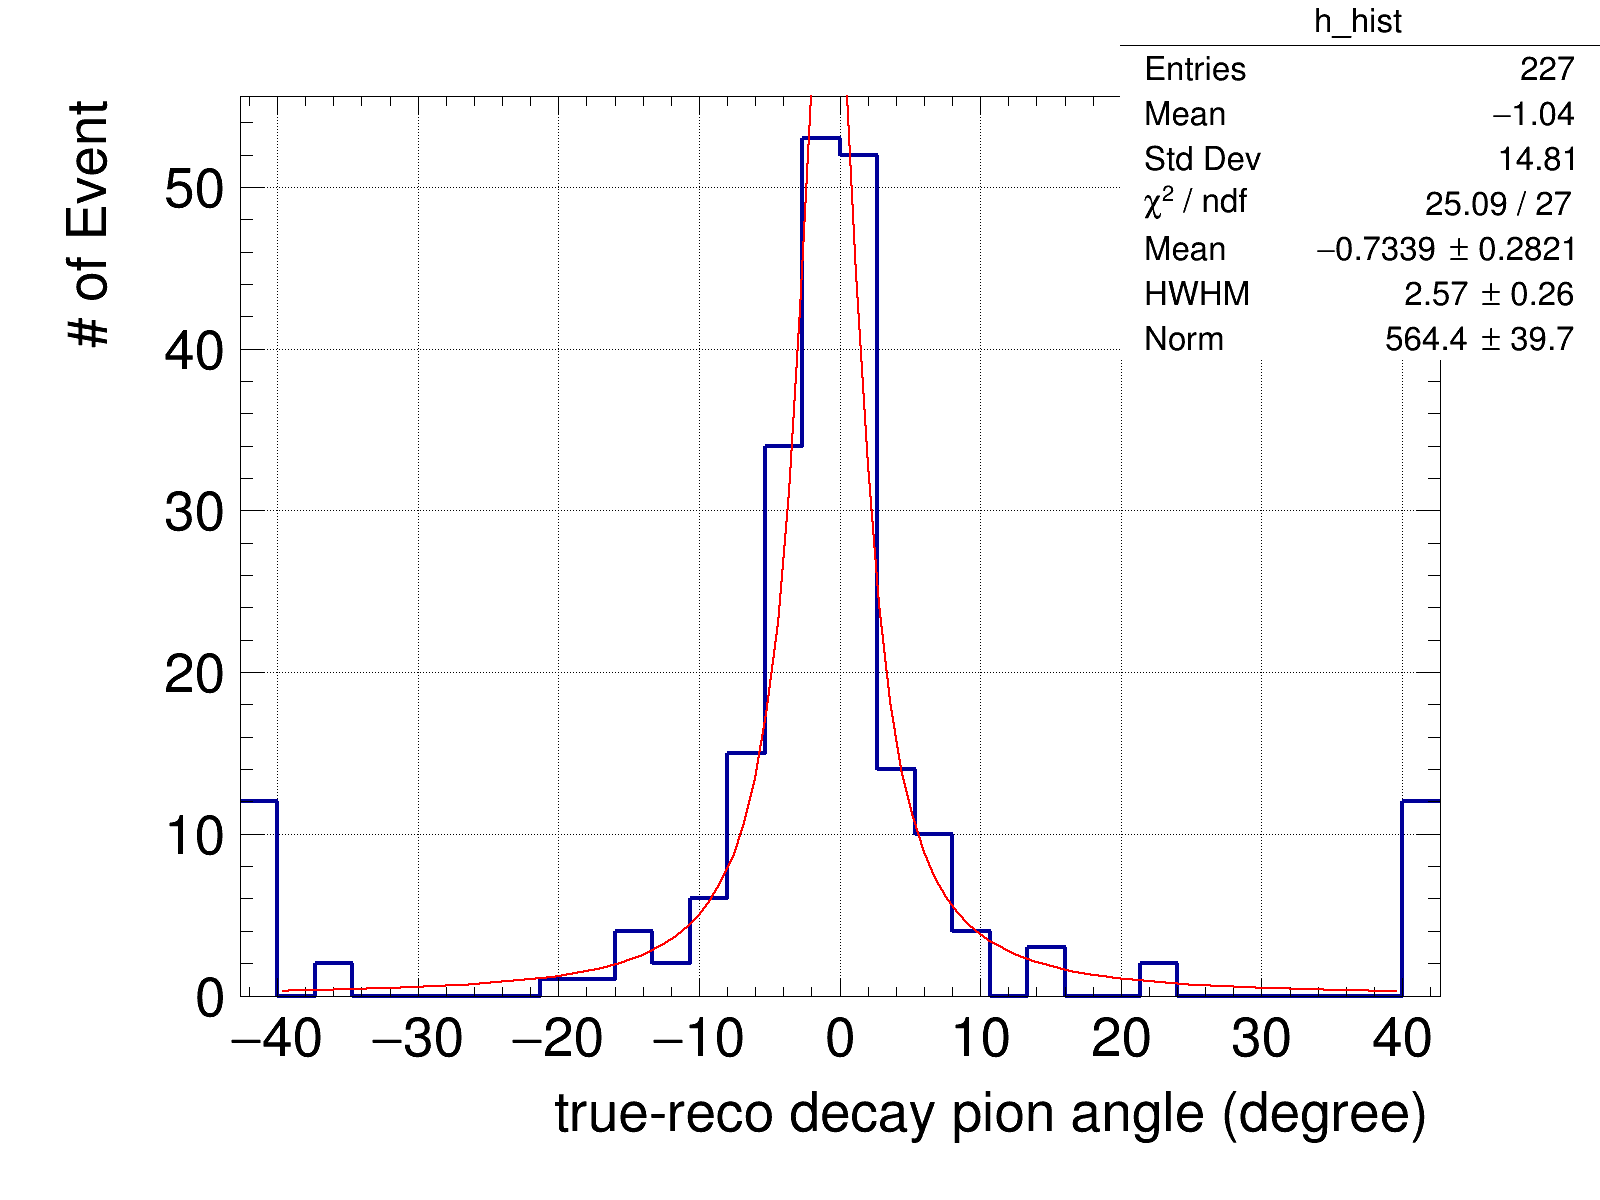
\includegraphics[width=\textwidth]{fig/SFGpTPCmu_dang_res_hist_al14.png}
            \caption{$\pidecang$ resolution.}
            \label{fig:1pi-decang-res}
       \end{subfigure}
       \begin{subfigure}{0.45\textwidth}
            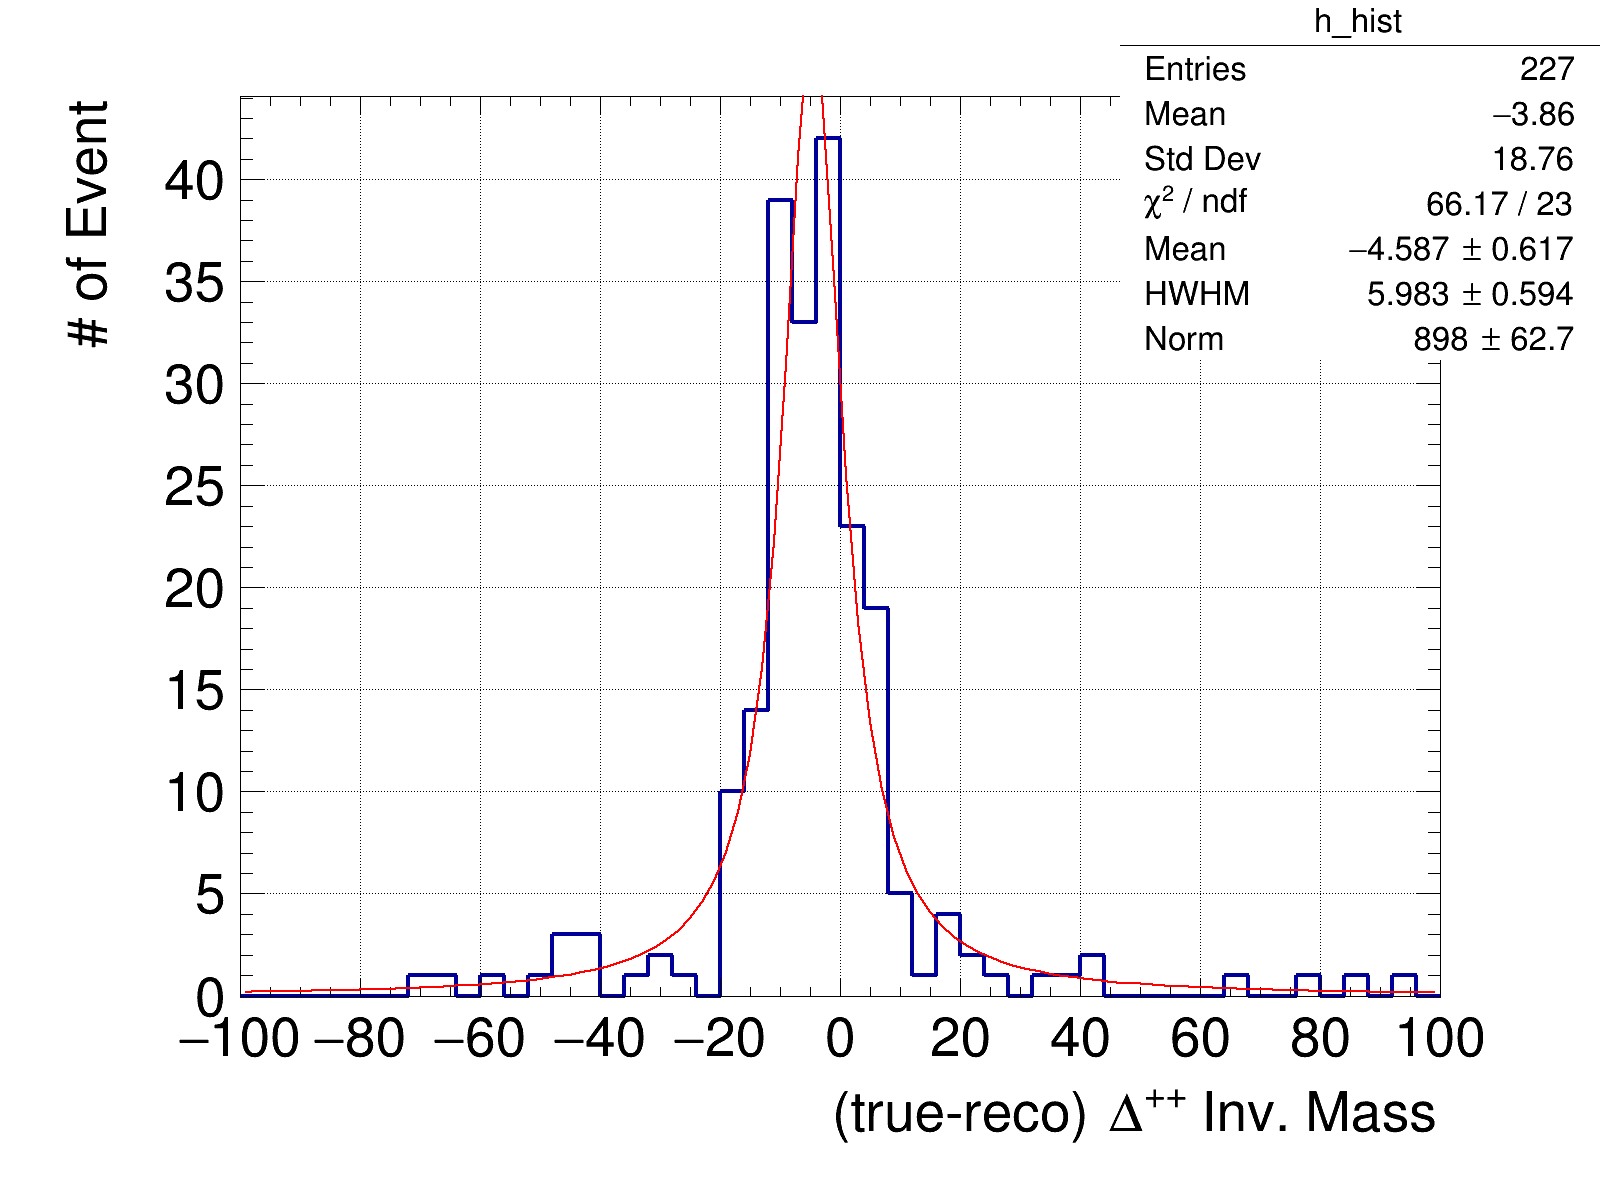
\includegraphics[width=\textwidth]{fig/SFGpTPCmu_edelta_res_hist_al14.png}
            \caption{$\mdeldec$ resolution.}
            \label{fig:1pi-mdel-res}
       \end{subfigure}
       \caption{COM reconstruction results.}
       \label{fig:1pi-com-res}
    \end{figure}
 

\minitoc